% !TEX encoding = UTF-8
\documentclass[a4paper,12pt]{article}
\usepackage[T1]{fontenc}
\usepackage[utf8]{inputenc}
\usepackage[italian]{babel}
\usepackage{color, colortbl}
\usepackage{graphicx}
\definecolor{Ash}{rgb}{0.7,0.75,0.71}
\usepackage{../Use-Case/tikz-uml}


\begin{document}

\title{\textbf{TrackMyCar - Live Positioning System}\\Documento di Caratteristiche}

\author{Kevin Mansoldo, Matteo Dal Monte, Luca Vicentini}
\date{}
\maketitle
\pagebreak

\tableofcontents
\pagebreak

\section{Lista Destinatari del Documento}

\begin{table*}[ht]
\begin{center}
\begin{tabular}{p{1cm} p{4.5cm} p{5cm} p{2cm}}
\rowcolor{Ash}
\hline
Copia & Persona & Organizzazione & Data \\ \hline
1 & Kevin Mansoldo & Azienda & Data \\ 
2 & Matteo Dal Monte & Azienda & Data \\ 
3 & Luca Vicentini & Azienda & Data \\ 
4 & Claudio Tomazzoli & Cliente & Data \\ \hline
\end{tabular}
\end{center}


\begin{center}
\begin{tabular}{p{6cm} p{5cm} p{2cm}}
\rowcolor{Ash}
\hline
Azione & Persona & Data \\ \hline
Documento redatto da & Kevin Mansoldo & Data \\ 
Documento approvato da & Matteo Dal Monte & Data \\ 
Documento approvato da & Luca Vicentini & Data \\ \hline
\end{tabular}
\end{center}
\end{table*}

\subsection{Versione Documento}
\begin{table*}[ht]
\begin{center}
\begin{tabular}{p{1cm} p{4.5cm} p{5cm} p{2cm}}
\rowcolor{Ash}
\hline
Versione & Autore & Note & Data \\ \hline
1.0 & Kevin Mansoldo & Stesura Iniziale & Data \\ 
1.1 & Kevin Mansoldo & Revisione su osservazioni del gruppo & Data \\ 
1.2 & Kevin Mansoldo & Revisione Finale & Data \\ \hline
\end{tabular}
\end{center}
\end{table*}

\subsection{Supporto Documento}
\begin{table*}[ht]
\begin{center}
\begin{tabular}{p{6cm} p{5cm} p{2cm}}
\rowcolor{Ash}
\hline
Nome File & Tipo & Estensione \\ \hline
Caratteristiche & Portable Document Format & .pdf \\ \hline
\end{tabular}
\end{center}
\end{table*}

\clearpage

\pagebreak

\section{Introduzione e Obiettivi}
Il documento di caratteristiche include le specifiche tecniche del progetto.

Al giorno d'oggi è fondamentale possedere un mezzo di trasporto proprio.
Dati gli alti costi di acquisto e gestione, è importante difendere il proprio investimento. Il modo migliore per farlo è possedere un sistema di sorveglianza adeguato che ci permetta di tracciare in ogni momento la posizione del nostro veicolo. Ciò si rende indispensabile in caso di furto.
Si intende quindi realizzare un software in grado di monitorare in tempo reale un veicolo (auto/moto) e garantire l’eventuale recupero in caso di furto.

\section{Definizioni, Acronimi e Abbreviazioni}

Per le definizioni di alcuni termini fondamentali, fare riferimento al glossario ``Glossario.pdf'' all'interno della documentazione di progetto.

\begin{table}[h]
\begin{center}
\begin{tabular}{ l  l  l } 
\rowcolor{Ash}	
\hline	
Nome File & Tipo File & Estensione  \\ \hline
Vision & Requisiti, Business Needs e Motivazioni & Vision.pdf  \\ 
Development Case & Linee guida di sviluppo del progetto & DevCase.pdf  \\ 
Glossario & Descrizione di termini specifici & Glossario.pdf  \\ \hline
\end{tabular}
\end{center}
\end{table}

\pagebreak

\section{Architettura}
Il sistema è composto di diverse componenti hardware e software, utili a fornire un funzionamento agevole  e un'ampia interoperabilità. \\
Tra queste possiamo annoverare: 
\begin{itemize}
\item Una centralina dotata di un modulo GSM, periferica GPS e input seriale per l'acquisizione dei contenuti multimediali.  Il modulo integrato deve essere collegato ad un sistema di alimentazione indipendente dalla batteria, in modo da garantire il funzionamento in qualunque occasione (es. rimozione batteria del veicolo).
\item Database Centralizzato per la memorizzazione dei dati.
\item Applicazione Web per la consultazione delle informazioni richieste.
\end{itemize}

Tale configurazione permette di mantenere la massima interoperabilità tra le parti, senza inficiare la semplicità di utilizzo.

\pagebreak

\subsection{Modello Logico}
Lo schema seguente mostra come viene regolato lo scambio di dati tra il modulo di TrackMyCar, il database e l'applicazione web per la gestione dei contenuti.\\

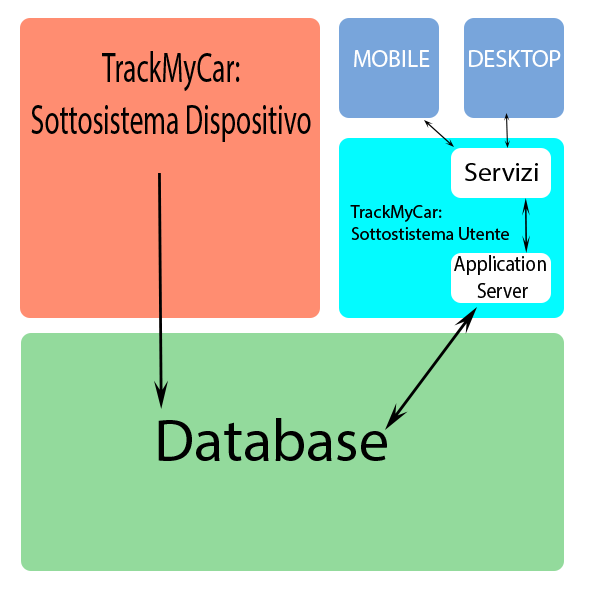
\includegraphics[scale=.65]{../IMG/ModLogico.png}
\pagebreak

\subsection{Modello Fisico}
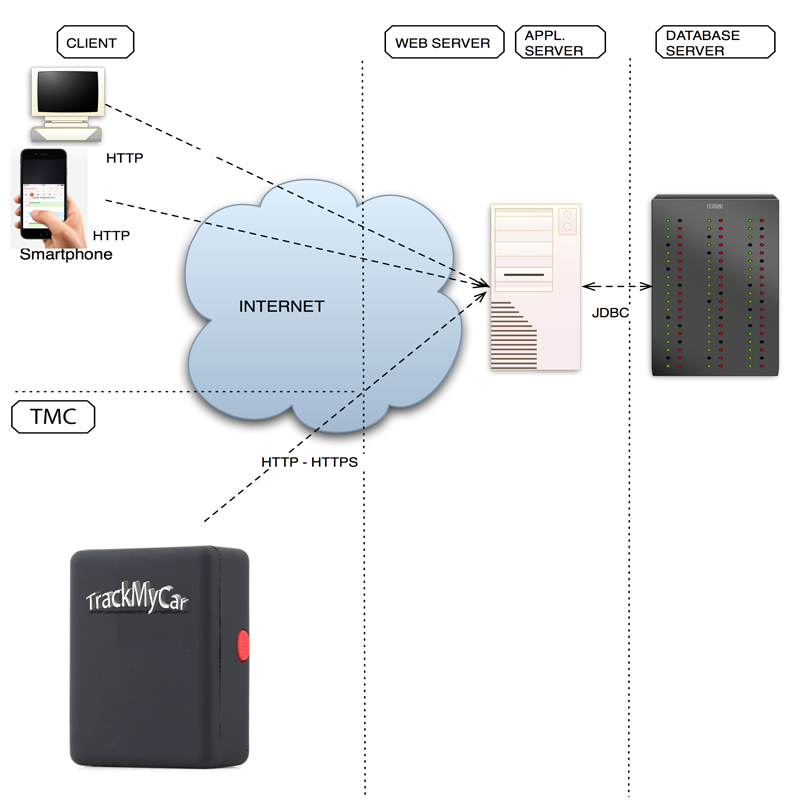
\includegraphics[width=12cm, height=12cm]{../IMG/ModFisico.png}


\subsection{Tecnologie}
\begin{table}[h]
Gli elementi tecnologici impiegati sono i seguenti:
\begin{center}
\begin{tabular}{ p{6,5cm}  p{6,5cm} }
\rowcolor{Ash}
\hline	
Tipo & Versione \\ \hline
Protocollo & TCP-IP \\ 
Ambiente & Java 2 Enterprise Edition \\ 
Sistema Operativo & Windows, Linux, Mac OS X \\ 
Motore Database & POSTGRESQL 9.4 \\ 
Application Server & Tomcat 7 \\ \hline
\end{tabular}
\end{center}
\end{table}

\pagebreak

\section{Requisiti Funzionali}
I requisiti funzionali disciplinano l'interazione dei vari soggetti con il sistema considerato. Se venissero violati, causerebbero la perdita di significato del progetto.

\begin{center}
\begin{tikzpicture}
\tikzumlset{fill usecase=white!10}

\umlusecase[x=2, y=4, width=5cm]{Gestione Utenti}
\umlusecase[x=2, y=2.5, width=5cm]{Gestione Veicoli}
\umlusecase[x=2, y=1, width=5cm]{Associazione Guidatore-Veicolo}
\umlusecase[x=2, y=-0.5, width=5cm]{Impostazione Allarmi}


\umlusecase[x=2, y=-3.5, width=5cm]{Visualizza posizione}
\umlusecase[x=2, y=-5, width=5cm]{Controllo Eccesso Velocità}
\umlusecase[x=2, y=-6.5, width=5cm]{Consultazione Storico Furti}
\umlusecase[x=2, y=-8, width=5cm]{Riproduzione Video}
\umlusecase[x=2, y=-9.5, width=5cm]{Visualizzazione Informazioni}

\umlactor[x=-4, y=1, scale=1.5]{Amministratore}
\umlassoc{Amministratore}{usecase-1}
\umlassoc{Amministratore}{usecase-2}
\umlassoc{Amministratore}{usecase-3}
\umlassoc{Amministratore}{usecase-4}


\umlactor[x=-4, y=-6.5, scale=1.5]{Regular}
\umlassoc{Regular}{usecase-5}
\umlassoc{Regular}{usecase-6}
\umlassoc{Regular}{usecase-7}
\umlassoc{Regular}{usecase-8}
\umlassoc{Regular}{usecase-9}

\umlinherit{Regular}{Amministratore}

\end{tikzpicture}
\end{center}

\pagebreak

\section{Requisiti Non Funzionali}
I requisiti non funzionali sono condizioni non esplicitamente dichiarate dal cliente, ma devono essere considerate in modo molto accurato per far sì che il sistema funzioni e risponda alle esigenze di utilizzo della vita comune, fornendo soluzioni per gli eventuali malfunzionamenti. 

\subsection{Robustezza}
Nel caso vi siano problemi nel salvare i dati nel Database, il sistema visualizza un messaggio di errore segnalando la causa. Nel caso non sia possibile visualizzare i dati richiesti da una particolare funzionalità, il sistema visualizza un messaggio di errore segnalando la causa. Nel caso in cui si voglia eliminare un dato esistente, viene chiesta la conferma; in caso negativo si abbandona l'operazione.
\subsection{Sicurezza}
L'accesso al sistema è regolato da identificazione dell'utente; le autorizzazioni a compiere determinate operazioni dipendono dal profilo con il quale si è connessi. Il profilo con maggiori autorizzazioni è quello dell’amministratore; nel sistema deve esisterne almeno uno.
Il traffico di dati in rete è criptato, dall’application server al database server tramite l’uso del protocollo JDBC, dal web server all’application server tramite l’uso del protocollo binario AJP; dal browser al web server è possibile usare il protocollo HTTPS.
\subsection{Prestazioni}
L’applicativo funziona tramite la generazione e lo scambio di pagine ipertestuali ovvero di informazioni ipertestuali che vengono visualizzate da un browser tramite protocollo HTTP. A prescindere dalla qualità e dalle condizioni di rete, il sistema restituisce le informazioni relative agli oggetti entro un tempo medio di 5 secondi; stesso tempo viene impiegato per la risposta alle interrogazioni della base di dati. Il refresh del tracking viene effettuato ogni secondo, ma può essere modificato in base alle richieste del cliente.
\pagebreak
\subsection{Interoperabilità}
\begin{itemize}
\item \textbf{Thin Client:} permette, grazie alla tecnologia HTML, di poter accedere al sistema tramite qualunque elaboratore dotato di browser HTML.
\item \textbf{Mobile Client:} è prevista la possibilità di accesso al sistema anche in mobilità.
\item \textbf{Server:} Avendo scelto la tecnologia Java, è possibile cambiare il sistema operativo del server a condizione che questo disponga di una JVM, senza influire sull'applicazione se non per i cambiamenti dei parametri derivanti dalle differenze nei file system.
\end{itemize}
\subsection{Portabilità}
\begin{itemize}
\item \textbf{Thin/Mobile Client:} permette, grazie alla tecnologia HTML, di poter accedere al sistema tramite qualunque dispositivo dotato di browser HTML.
\item \textbf{Server:} Avendo scelto la tecnologia Java, è possibile cambiare il sistema operativo del server a condizione che questo disponga di una JVM, senza modifiche o ricompilazioni.
\end{itemize}
\subsection{Scalabilità}
Essendo il nostro sistema basato su Java Enterprise Edition, architettura altamente scalabile, in caso di numero elevato di utenti sarà possibile servire le richieste tramite una semplice clonazione dell'application server e una configurazione adeguata del load balancing, senza ulteriori interventi sul software.
\pagebreak

\section{Funzioni per l'utente}
Gli attori di questo sistema sono due:
\begin{itemize}
\item Amministratore
\item Regular
\end{itemize}

Di seguito verranno elencate le funzioni disponibili per i vari attori, dove si assume che per \textit{gestione} si intendano inserimento, modifica e cancellazione.

\subsection{Funzioni Amministratore}
Un amministratore gestisce i dati relativi agli utenti, ai gruppi ed alle funzioni ed i permessi ad operare. Può inoltre gestire l'associazione dei veicoli ai rispettivi utilizzatori, gli allarmi e le notifiche via SMS e mail. Tutte le funzioni disponibile per il Regular possono comunque essere svolte dall'amministratore.
\begin{center}
\begin{tikzpicture}
\tikzumlset{fill usecase=white!10}

\umlusecase[x=2, y=4, width=5cm]{Gestione Utenti}
\umlusecase[x=2, y=2.5, width=5cm]{Gestione Veicoli}
\umlusecase[x=2, y=1, width=5cm]{Associazione Guidatore-Veicolo}
\umlusecase[x=2, y=-0.5, width=5cm]{Impostazione Allarmi}


\umlactor[x=-4, y=1, scale=1.5]{Amministratore}
\umlassoc{Amministratore}{usecase-1}
\umlassoc{Amministratore}{usecase-2}
\umlassoc{Amministratore}{usecase-3}
\umlassoc{Amministratore}{usecase-4}


\end{tikzpicture}
\end{center}

\pagebreak

\subsection{Funzioni Regular}
Le funzioni di un regular user riguardano la consultazione di informazioni relative al veicolo tracciato, come schematizzato in seguito.
\begin{center}
\begin{tikzpicture}
\tikzumlset{fill usecase=white!10}

\umlusecase[x=2, y=-3.5, width=5cm]{Visualizza posizione}
\umlusecase[x=2, y=-5, width=5cm]{Controllo Eccesso Velocità}
\umlusecase[x=2, y=-6.5, width=5cm]{Consultazione Storico Furti}
\umlusecase[x=2, y=-8, width=5cm]{Riproduzione Video}
\umlusecase[x=2, y=-9.5, width=5cm]{Visualizzazione Informazioni}


\umlactor[x=-4, y=-6.5, scale=1.5]{Regular}
\umlassoc{Regular}{usecase-5}
\umlassoc{Regular}{usecase-6}
\umlassoc{Regular}{usecase-7}
\umlassoc{Regular}{usecase-8}
\umlassoc{Regular}{usecase-9}

\end{tikzpicture}
\end{center}


\section{Specifiche sulle interfacce esterne}
\subsection{Input}
\begin{itemize}
\item \textbf{Thin/Mobile Client:} permette, grazie alla tecnologia HTML, di poter accedere al sistema tramite qualunque dispositivo dotato di browser HTML.
\item \textbf{TrackMyCar:} I dati vengono trasmessi al server centrale tramite protocollo criptato HTTPS.
\end{itemize}
\subsection{Output}
\begin{itemize}
\item \textbf{Thin/Mobile Client:} I dati vengono trasmessi dal server al dispositivo dell'utente tramite interfacce HTML. La stampa avviene tramite browser web.
\item \textbf{Telefono Cellulare:} Le notifiche vengono inoltrate tramite SMS e/o mail.
\item \textbf{TrackMyCar:} I dati vengono trasmessi dal server centrale al dispositivo tramite protocollo criptato HTTPS.
\end{itemize}

\pagebreak

\section{Standard e documentazione a supporto}
\subsection{Standard}
\begin{itemize}
\item Tecnologia GPS
\item J2EE
\end{itemize}

\subsection{Documentazione}

A supporto dell'applicativo saranno realizzati un Manuale Utente in formato elettronico, consultabile e scaricabile dal sito del prodotto.
\pagebreak
\end{document}